%
% Tesi D.S.I. - modello preso da
% Stanford University PhD thesis style -- modifications to the report style
%
%%%%%%%%%%%%%%%%%%%%%%%%%%%%%%%%%%%%%%%%%%%%%%%%%%%%%%%%%%%%%%%%%%%%%%%%%%%
%                                                                         %
%			TESI DOTTORATO                                                   %
%			______________                                                   %
%                                                                         %
%			AUTORE: Elena Pagani                                             %
%                                                                         %
%			Ultima revisione: 7.X.1998                                       %
%                                                                         %
%%%%%%%%%%%%%%%%%%%%%%%%%%%%%%%%%%%%%%%%%%%%%%%%%%%%%%%%%%%%%%%%%%%%%%%%%%%
%
%
\documentclass[12pt]{report}
%    \renewcommand{\baselinestretch}{1.6}      % interline spacing
%
% \includeonly{}
%
%			PREAMBOLO
%
\usepackage[a4paper]{geometry}
\usepackage{amssymb,amsmath,amsthm}
\usepackage{graphicx}
\usepackage{url}
\usepackage{hyperref}
\usepackage{epsfig}
\usepackage[italian]{babel}
\usepackage{tesi}
\usepackage{float}
% per le accentate
\usepackage[T1]{fontenc}
\usepackage[utf8]{inputenc}
\usepackage{hyperref}
%
\newtheorem{myteor}{Teorema}[section]
%
\newenvironment{teor}{\begin{myteor}\sl}{\end{myteor}}
%
%
%			TITOLO
%
\begin{document}
\begin{center}
	
\includegraphics[height=3.0cm]{logo_unimi.png}
\end{center}

\title{Sviluppare il pensiero computazionale con i quesiti Bebras: approcci e strumenti per l'uso nella pratica scolastica.}
\author{Annalisa CALCAGNI}
\dept{Corso di Laurea Magistrale in Informatica } 
\anno{2016-2017}
\matricola{865610}
\relatore{Prof. Violetta LONATI}
\correlatore{Prof. Mattia MONGA}
%
%        \submitdate{month year in which submitted to GPO}
%		- date LaTeX'd if omitted
%	\copyrightyear{year degree conferred (next year if submitted in Dec.)}
%		- year LaTeX'd (or next year, in December) if omitted
%	\copyrighttrue or \copyrightfalse
%		- produce or don't produce a copyright page (false by default)
%	\figurespagetrue or \figurespagefalse
%		- produce or don't produce a List of Figures page
%		  (false by default)
%	\tablespagetrue or \tablespagefalse
%		- produce or don't produce a List of Tables page
%		  (false by default)
% 
%			DEDICA
%
\beforepreface
        {\hfill \Large {\sl dedicato a \dots}}
% 
\afterpreface
%			PREFAZIONE: Introduzione
%
\prefacesection{Introduzione}
hkjafgyruet
%
%
%
% 
% 
%			CAPITOLO 1: Bebras
\chapter{Bebras}
\label{cap1}
%
\section{Bebras a livello mondiale}
Negli ultimi dieci anni in tutto il mondo sono state organizzate numerose gare riguardanti l'Informatica, principalmente per due motivi: selezionare studenti particolarmente talentuosi in questo campo, come accade nelle Olimpiadi Informatiche, oppure diffondere fin dalle prime fasi dell'educazione i concetti base di questa disciplina scientifica che spesso nelle scuole si finisce per confondere con le "applicazioni" dell'Informatica. Quest'ultimo è esattamente lo scopo del Bebras, il quale è una gara organizzata annualmente dal 2004 in più paesi (50 nel 2016), con un numero di partecipanti superiore a mezzo milione nelle ultime edizioni.\cite{BellettiniITICSE2015}
Bebras ("castoro" nella lingua del Paese, la Lituania, dove è nata l'iniziativa) è un'organizzazione internazionale che ha lo scopo di promuovere nelle scuole gli aspetti scientifici dell'informatica. I giochi Bebras sono accessibili agli studenti delle scuole primarie e secondarie anche senza nessuna specifica conoscenza pregressa. Gli studenti partecipano a questa gara attraverso il computer direttamente dalle proprie scuole, sotto la supervisione di un loro insegnante, il quale successivamente può integrare la correzione della suddetta gara all'interno delle attività curricolari.

La gara Bebras è composta da quesiti di due tipi: domande a scelta multipla con quattro risposte e problemi interattivi. Il numero di quesiti varia da un anno all'altro: da diciotto a ventiquattro domande di difficoltà diverse, da risolvere in 40, 45 o 55 minuti.
Il Bebras è organizzato annualmente a livello locale, dalla delegazione del Paese partecipante, la quale utilizza tecnologie diverse per l'esecuzione della gara, ma generalmente tutti usano sistemi di gestione online.
Ogni delegazione sceglie, da un insieme di quesiti approvati dalla comunità internazionale, quelli da inserire nella loro edizione locale del Bebras, ma alcuni di essi sono da utilizzare obbligatoriamente.
\newpage
I quesiti sono divisi in sei categorie:
\begin{itemize}
\item Pre-Primary: 5-8 anni
\item Primary: 8-10 anni
\item Benjamins: 10-12 anni
\item Cadets: 12-14 anni
\item Juniors: 14-16 anni
\item  Seniors: 16-19 anni
\end{itemize}
Ogni delegazione locale può riorganizzare le proprie categorie a seconda delle proprie realtà scolastiche.
\\

Il cuore dell'organizzazione di questa gara è un workshop annuale internazionale che riunisce delegati provenienti da tutti i Paesi coinvolti, con lo scopo di proporre e correggere i quesiti da sottoporre ai partecipanti.  
Ogni Paese partecipante è invitato a fornire almeno un mese prima del workshop un insieme di proposte di quesiti, che sono resi disponibili per essere visionati e commentati. Durante i tre giorni di lavoro, i partecipanti vengono divisi in gruppi ad ognuno dei quali viene assegnato un insieme di quesiti su cui discutere. Alla fine dei giorni di lavoro ogni gruppo proporrà una serie di quesiti candidati ad essere quelli obbligatori, ma diverranno tali solo dopo la votazione finale di ogni partecipante.

Ogni delegazione locale sceglie tra tutti i quesiti redatti nel workshop quelli che saranno utilizzati per la competizione locale e quindi tradotti adeguatamente nella propria lingua.
I quesiti Bebras sono indipendenti da attività specifiche curricolari e si evita il gergo specifico informatico, infatti ci si concentra su ciò che è chiamato il pensiero computazionale (Computational Thinking) che risulta essere utile a tutti indipendentemente dalle personali inclinazioni. I problemi proposti, infatti, presentano reali situazioni informatiche che richiedono di interpretare informazioni, manipolare strutture discrete, elaborare dati e ragionare algoritmicamente.
%
%
\section{Quesiti Bebras}
I quesiti Bebras sono molto importanti sia per i partecipanti alla gara, sia per i docenti; infatti i primi dovrebbero essere spinti a pensare in maniera "informatica" e i secondi dovrebbero riflettere su come rendere affascinante il programma scolastico di questa disciplina. \'{E} quindi fondamentale creare dei quesiti creativi e interessanti che possano attirare l'attenzione degli studenti e allo stesso tempo insegnare l'informatica come scienza e non come strumento tecnologico.
Tali quesiti trattano concetti di informatica come algoritmi e programmi(sequenziali e concorrenti), strutture dati(heaps, pile, stack), modellizzazione di stati(flusso di controllo, flusso di dati), interazione uomo-computer, etc.

Un aspetto fondamentale dei quesiti Bebras è che siano ben formulati, la comunità internazionale infatti presta molta attenzione a riguardo.

Un "buon quesito" deve essere:
\begin{itemize}
	\item riguardante un concetto informatico
	\item facilmente comprensibile
	\item risolvibile in 3 minuti
	\item corto, cioè visibile per intero sullo schermo in un'unica pagina
	\item risolvibile al computer senza l'uso di altri software o fogli e matita
	\item indipendente da specifici sistemi
	\item interessante e divertente
\end{itemize}
Lo scopo principale è quello di focalizzarsi sulla comprensione di princìpi, idee e concetti coinvolti nell'informatica cercando di presentare dati e situazioni reali in cui gli studenti possono immedesimarsi.

Un altro aspetto fondamentale è assegnare la corretta difficoltà delle attività, altrimenti si potrebbe lasciare ai partecipanti la percezione che la gara risulti essere o troppo semplice o troppo difficile e quindi poco accattivante.
Non essendo facile valutare la difficoltà di un quesito, è molto utile fare delle analisi sulle prestazioni dei partecipanti dopo la conclusione del concorso così da poter migliorare le scelte e le strategie future.
\\
Di seguito viene riportato un tipico quesito Bebras dell'edizione italiana: si può notare che non vengono richieste conoscenze pregresse, ma lo scopo è che gli studenti scoprano i concetti informatici attraverso divertenti problemi.
\\
\begin{figure}[H]
	\centering
	\fbox{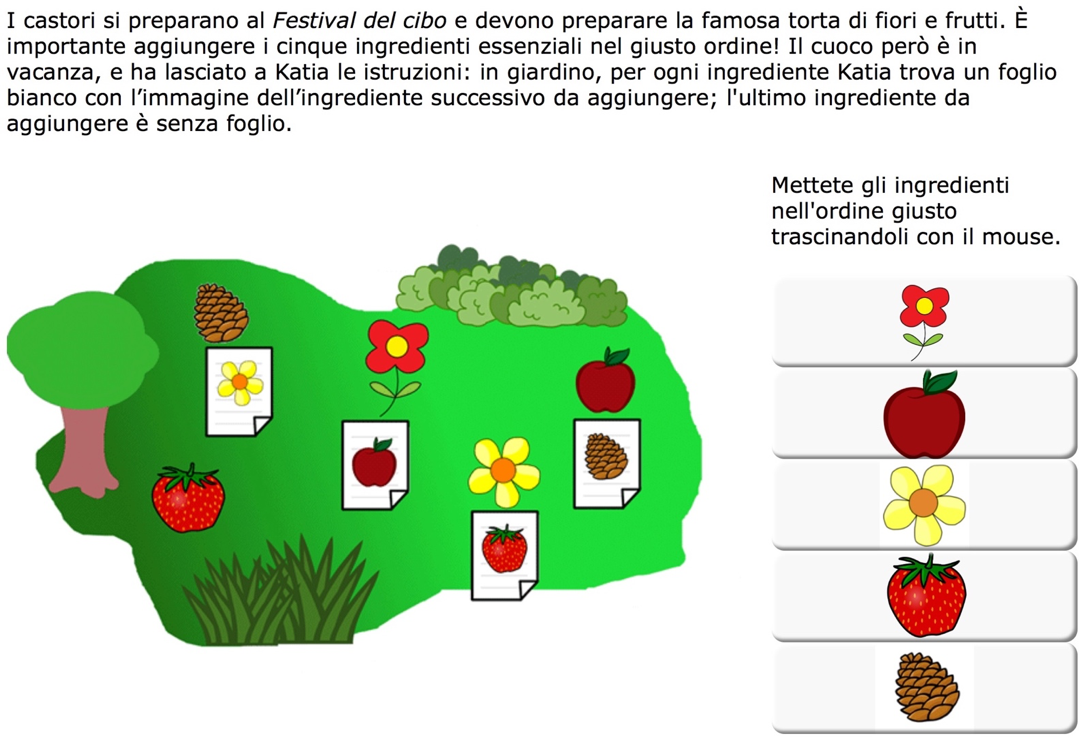
\includegraphics[height=10.0cm]{2016-HU-02Testo.png}}
	\caption{La ricetta segreta (2016-HU-02)}\label{fig:1}
\end{figure}
Questo quesito era presente nella gara svolta nel novembre 2016, all'interno della categoria KiloBebras.

La lista degli ingredienti è un esempio della struttura dati chiamata lista. Il foglio che indica l'ingrediente successivo costituisce il puntatore all'elemento successivo della lista. Per accedere alla lista occorre avere il puntatore al primo elemento della lista.
%
%
%
\\
\begin{figure}[H]
	\centering
	\fbox{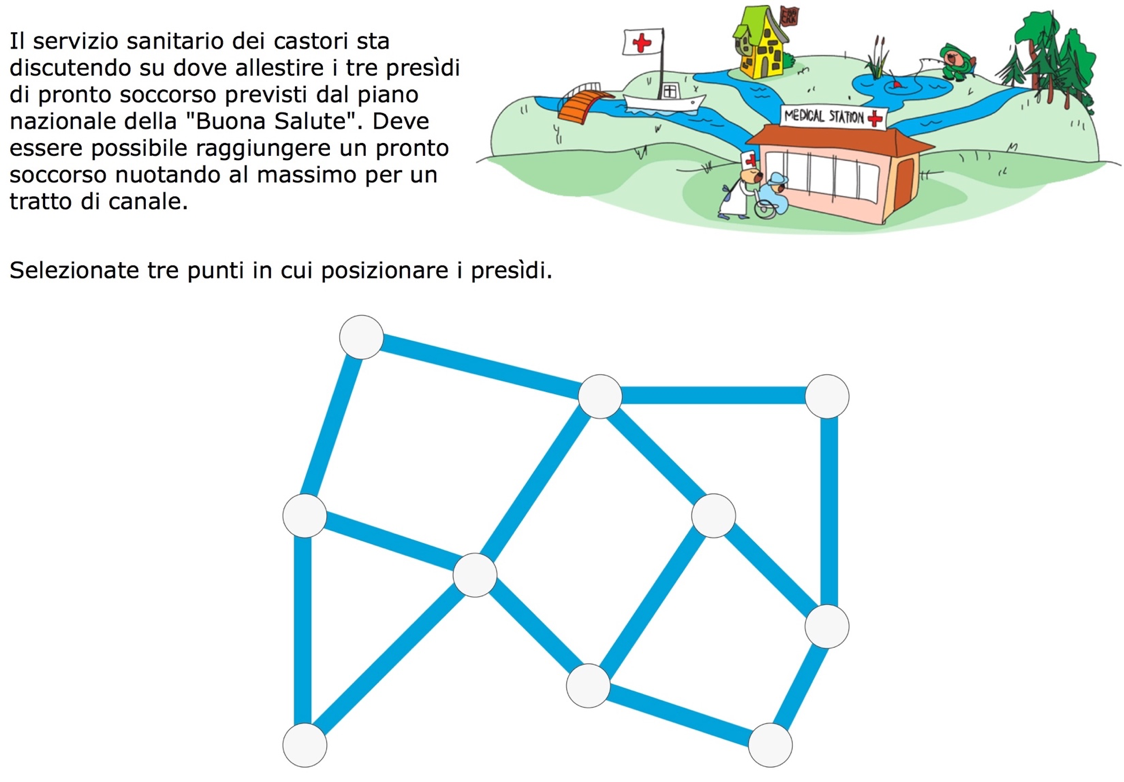
\includegraphics[height=10.0cm]{2016-CH-03Testo.png}}
	\caption{Pronto soccorso (2016-CH-03)}\label{fig:2}
\end{figure}
Questo quesito era presente nella gara svolta nel novembre 2016, all'interno della categoria MegaBebras, GigaBebras e TeraBebras.

La rete di canali raffigurata può essere rappresentata da un grafo, in cui i tratti di canale sono gli archi (non orientati, cioè percorribili in entrambi i sensi) e i punti dove essi si incontrano sono i nodi. Il quesito proposto è un esemplare del problema dell’insieme dominante nella versione in cui si tratta di decidere se un insieme dominante esiste. 

\section{Classificazione quesiti}
Dalla nascita del Bebras, nel 2004, fino ad oggi sono stati redatti un numero ingente di quesiti. All'interno della comunità è quindi nata l'esigenza di classificarli per poter creare quesiti più eterogenei ed equilibrati rispetto ai concetti trattati.

La prima classificazione dei quesiti all'interno della comunità Bebras che è stata proposta nel 2008 da Dagiene e Futschek\cite{DagieneISEEP2008}, consiste nelle seguenti categorie:
\begin{itemize}
\item \textbf{comprensione dei dati}
attraverso la rappresentazione simbolica, numerica e visiva, la codifica, la crittografia

\item \textbf{ragionamento algoritmico},
compresi gli aspetti di programmazione

\item \textbf{uso di sistemi informatici}
come motori di ricerca, email, fogli elettronici; principi generali senza riferimento ad uno specifico sistema

\item \textbf{strutture, patterns e ottimizzazione combinatoria}
come i grafi

\item \textbf{puzzles}
come giochi logici

\item \textbf{l'Informatica e la società}
includendo argomenti sociali, etici e culturali riguardanti la disciplina informatica
\end{itemize}

Tale classificazione, nonostante sia stata utilizzata per molto tempo, è risultata troppo generica per essere applicata alla grande varietà di quesiti Bebras, inoltre alcune categorie spesso non vengono utilizzate perché molto legate ad aspetti non attinenti agli attuali quesiti Bebras.
Successivamente nel 2009 è stata proposta da Kalas e Tomcsanyiova\cite{KalasIFIP2009} un'altra tecnica di classificazione basata sugli argomenti informatici trattati, ogni quesito poteva essere inserito in una o due categorie:
\begin{itemize}
	\item \textbf{alfabetizzazione digitale}: conoscenze di base, concetti di informatica, uso del computer, questioni etiche e legali, sicurezza, storia dell'informatica
	\item \textbf{programmazione}: descrizione formale di una soluzione, di un processo o di un comportamento; comprensione, analisi, interpretazione di una descrizione; algoritmi e pensiero algoritmico
	\item \textbf{risoluzione di un problema}: ragionamento logico e argomentazione; puzzles, enigmi e problemi; strategie per la soluzione dei problemi
	\item \textbf{gestione dei dati}: rappresentazioni di dati, codifiche, patterns, strutture dati
\end{itemize}

Più recentemente, nel 2015, è stata proposta da Pohl e Westmeyer \cite{PohlLNCS2015} una classificazione gerarchica basata sull'idea principale di Schwill \cite{SchwillEATCS1994}.
I nodi-padre di tale gerarchia proposta sono:
\begin{itemize}
	\item \textbf{algoritmizzazione}: concetti di programmazione, valutazione della complessità, verifica della correttezza, processi concorrenti, ... 
	\item \textbf{organizzazione strutturale}: modularizzazione, gerarchizzazione, ortogonalizzazione
	\item \textbf{formalizzazione}: sintassi e semantica
	\item \textbf{sistemi informatici}: applicazioni informatiche
\end{itemize}

\'{E} stata proposta tale struttura gerarchica per permettere una classificazione a grana fine e su livelli di dettaglio diversi.

In seguito è stata presentata una classificazione ortogonale \cite{DagieneKEYCIT2015} a partire dalla Tassonomia di Bloom.
Quest'ultima è uno dei modi di formalizzare le fasi di acquisizione di informazioni attraverso la classificazione degli scopi educativi. In particolare i settori della tassonomia di Bloom fanno riferimento ai vari obiettivi che gli educatori dovrebbero definire per i loro studenti. Tali obiettivi sono divisi in tre domin\^{i}: cognitivo, affettivo e psicomotore. All'interno di tali domin\^{i}, il passaggio al livello successivo è pregiudicato dall'acquisizione delle conoscenze e abilità che precedono.
Questa tassonomia, insieme alla classificazione di Kalas precedentemente esposta \cite{KalasIFIP2009}, genera la seguente classificazione ortogonale:
\begin{itemize}
	\item Ricordare fatti generali, concetti di base
	\item Comprensione semplice di un dato linguaggio, di comandi e del loro significato
	\item Comprensione complessa della descrizione di processi, di regole e di metodi
	\item Applicare delle regole generative o metodi ad uno stato iniziale o input
	\item Interpretare date istruzioni o programmi
	\item Analizzare condizioni o processi
	\item Analizzare le corrispondenze di più descrizioni con più comportamenti
	\item Analizzare diverse situazioni o soluzioni in base a dati criteri
	\item Dedurre un possibile risultato, uno stato finale o un prodotto finale
	\item Mettere insieme informazioni
\end{itemize}

Nel 2017 vengono proposte due nuove classificazioni basate sulla definizione operazionale del pensiero computazionale sviluppata dall'ISTE (International Society for Technology in Education) e dal CSTA (Computer Science Teachers Association) \cite{flayerCT}.

La prima classificazione \cite{DagieneINFORMATICA2017} è composta da due dimensioni, nello specifico la dimensione delle abilità del pensiero computazionale e quella rappresentante i concetti informatici.
\newpage
La prima dimensione è così costituita:
\begin{itemize}
	\item \textbf{astrazione}: rimuovere dettagli non necessari, riconoscere elementi chiave, scegliere la rappresentazione di un sistema
	\item \textbf{pensiero algoritmico}: ragionare in termini di sequenze e di regole, eseguire un algoritmo, creare un algoritmo
	\item \textbf{scomposizione}: decomporre in sottoproblemi, ragionare su un problema in termini di sottoproblemi
	\item \textbf{valutazione}: trovare la soluzione migliore, prendere buone decisioni riguardo l'uso di risorse a disposizione
	\item \textbf{generalizzazione}: identificare patterns, risolvere nuovi problemi sulla base di problemi già risolti, utilizzare soluzioni generali in una specifica circostanza
\end{itemize}

La seconda dimensione è così definita:
\begin{itemize}
	\item \textbf{algoritmi e programmazione}: algoritmi, ricerca binaria, algebra booleana, etc.
	\item \textbf{dati, strutture dati, rappresentazione dati}: array, database, grafi, liste, code, etc.
	\item \textbf{processi e hardware}: deadlock, processamento di immagini, macchina di Turin, etc.
	\item \textbf{comunicazione e rete}: client/server, crittografia, protocolli, sicurezza, etc.
	\item \textbf{interazione, sistemi e società}: uso del computer, etica, virus, etc.
\end{itemize}

Si ottiene, quindi, una matrice bidimensionale in cui ogni quesito può essere posto in una sola categoria di concetti informatici ma in più categorie rappresentanti le abilità del pensiero computazionale.
\begin{figure}[H]
	\centering
	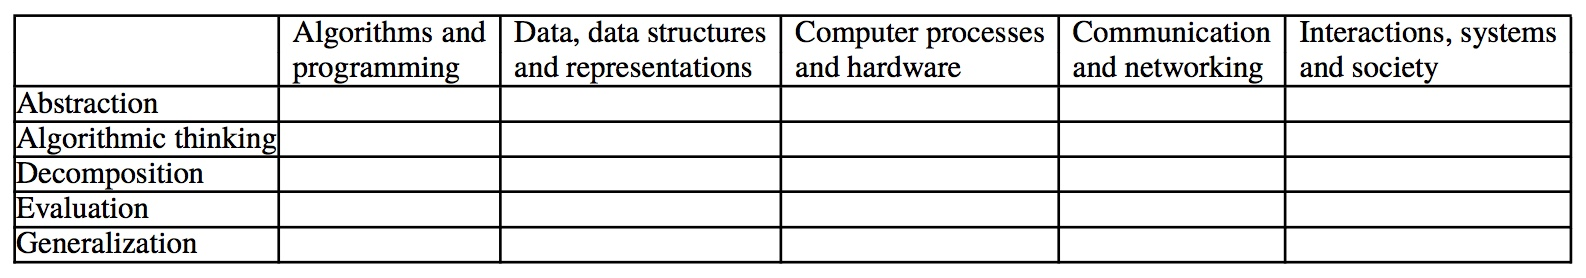
\includegraphics[height=2.7cm]{two-dimensional_classification.jpeg}
	\caption{Classificazione a due dimensioni}\label{fig:3}
\end{figure}

Infine la seconda classificazione \cite{LonatiITICSE2017}, che si basa anch'essa sulla definizione di pensiero computazionale definito dall'ISTE e dal CSTA, ha come obiettivo principale evidenziare il potenziale didattico dei quesiti Bebras.
Si vuole rendere comprensibile la classificazione anche a docenti senza una formazione informatica, inoltre tale approccio evidenzia le abilità cognitive coinvolte in un quesito e quindi il suo potenziale educativo.

Questa classificazione è così composta:
\begin{itemize}
	\item \textbf{Organizzazione logica dei dati}: organizzazione dei dati secondo certi criteri fissati (come ad esempio in una tabella), uso di strutture per rendere i dati più facili da elaborare, organizzare i dati in modo che godano di proprietà interessanti come nel caso della crittografia o della compressione dei dati.
	\item \textbf{Analisi logica dei dati}: “problemi logici” che si basano sul ragionamento logico-deduttivo e che chiedono di trarre conclusioni relative ai dati presentati nel quesito, quesiti che richiedono di osservare attentamente gli oggetti coinvolti (es: per riconoscere elementi simili o ricorrenti) o di procedere in maniera sistematica per stabilire se i dati del problema soddisfano o meno certe proprietà.
	\item \textbf{Rappresentazione digitale dell'informazione}: rappresentazione simbolica dei dati, rappresentazione visuale tramite diagrammi come istogrammi o grafici, strutture di dati che consentono di rappresentare proprietà interessanti (ad esempio: relazioni binarie o gerarchiche tra oggetti).
	\item \textbf{Pensiero algoritmico}: uso di metodi sistematici o procedure passo-passo, andando oltre la pura idea intuitiva su come risolvere il problema, ad esempio tramite la scomposizione del problema in sotto-problemi; la combinazione di operazioni elementari per svolgere un compito più complesso; l’uso di procedure formali (da eseguire o di cui calcolare/prevedere il risultato); l’applicazione di regole di transizione ad un sistema che si trova in un certo stato di partenza, ecc.
	\item \textbf{Identificare strategie risolutive}: ricerca di strategie algoritmiche non scontate per risolvere un problema.
	\item \textbf{Analizzare soluzioni algoritmiche}: quesiti che riguardano le caratteristiche generali di un algoritmo o di un metodo risolutivo presentato nel quesito, quali la correttezza del metodo o la sua praticabilità, quesiti che si ispirano a problemi di ottimizzazione, in cui si cerca la soluzione “migliore” tra tutte le soluzioni accettabili.
	\item \textbf{Implementare soluzioni algoritmiche}: problemi di programmazione o “coding”, si concentrano sull’implementazione di algoritmi attraverso l’uso di una sintassi formale definita nel quesito.
\end{itemize}

%
\section{Il Bebras in Italia}
Ogni delegazione della comunità internazionale del Bebras, come detto nella sezione 1, cura lo svolgimento della gara in locale.
In Italia il Bebras si svolge in un tempo massimo di 45 minuti attraverso una piattaforma su computer, nella settimana fissata dalla comunità internazionale, solitamente nel mese di novembre. Tali gare vengono proposte agli studenti dividendoli in gruppi da quattro componenti, infatti lavorare in squadra è un aspetto fondamentale.
Ogni gara è composta da 15 quesiti, diversamente dalle altre delegazioni Bebras, in Italia vengono proposti pochi quesiti con domande a risposta multipla. I quesiti scelti per l'edizione italiana sono in maggior parte domande interattive o domande che richiedono una complessa combinazione di risposte. Viene considerato anche un punteggio parziale per alcuni quesiti e non ci sono penalità per eventuali risposte errate.

In ogni categoria i quesiti sono divisi in tre livelli di difficoltà, ognuno dei quali corrisponde all'incremento di punti che possono essere accumulati.
Alcuni quesiti sono ripetuti in più categorie ma con un diverso livello di difficoltà e quindi una differente assegnazione di punteggio. In particolare l'intenzione degli organizzatori è che ogni categoria possa avere una coppia di quesiti che siano accessibili a tutti e una coppia in cui è richiesto un maggiore ragionamento. 

I partecipanti sono divisi in categorie in relazione alla classe frequentata:
\begin{itemize}
	\item \textbf{KiloBebras}: alunni delle Scuole Primarie [8-10 anni circa]
	\item \textbf{MegaBebras}: alunni delle classi prima e seconda delle Scuole Secondarie di primo grado [10-12 anni circa]
	\item \textbf{GigaBebras}: alunni delle classi terze delle Scuole Secondarie di primo grado [12-13 anni circa]
	\item \textbf{TeraBebras}: alunni del biennio delle Scuole Secondarie di secondo grado [13-15 anni circa]
	\item \textbf{PetaBebras}: alunni del triennio delle Scuole Secondarie di secondo grado [15-18 anni circa]
\end{itemize}

Ogni docente è invitato a discutere la correzione dei quesiti in classe  come occasione per approfondire o chiarire gli argomenti trattati. Spesso i docenti stessi richiedono la presenza di alcuni rappresentanti della delegazione italiana Bebras per poter svolgere la correzione insieme. Quest'ultima diventa un'occasione non solo per i partecipanti ma anche per gli stessi organizzatori che possono rilevare e osservare alcune criticità dell'edizione svolta e successivamente riflettere su eventuali correzioni per gli anni successivi.
A tal proposito la delegazione italiana ha svolto delle interviste \cite{LonatiKoli2017} in nove classi (circa 180 studenti) che hanno partecipato al Bebras nel 2016 con l'obiettivo di raccogliere commenti e individuare le difficoltà incontrate nella gara. 
A partire dalle osservazioni rilevate, sono stati modificati alcuni quesiti e riproposti a nuove classi per verificarne la correzione effettuata.


%			CAPITOLO 2: Indicazioni nazionali e Bebras
\chapter{Indicazioni nazionali e Bebras}
\label{cap2}
%%%%%%%%%%%%
\section{Perchè l'informatica nella scuola}
L'insegnamento dell'informatica è molto importante come scienza nelle scuole per i seguenti motivi \cite{InformaticaScuola}:
\begin{itemize}
	\item \textit{incrementa la creatività} grazie ai numerosi metodi che offre per affrontare e risolvere un problema
	\item \textit{sviluppa la costruttività} grazie alla progettazione di algoritmi che porta ad un'attività ingegneristica che produce risultati visibili
	\item \textit{aiuta a padroneggiare la complessità}, infatti affrontare problemi informatici aiuta a risolvere problemi più complessi riguardanti altre aree
	\item \textit{potenzia il ragionamento accurato} attraverso la scrittura di programmi in cui è necessaria l'esattezza in ogni minimo dettaglio
\end{itemize}
Quindi il ruolo dell'informatica nella scuola primaria e secondaria, come quello della matematica, è duplice: sia \textit{pratico}, infatti qualsiasi lavoro svolgeranno in futuro gli studenti, la componente digitale sarà importante; sia \textit{formativo}, l'informatica è infatti un valido strumento intellettuale per sviluppare abilità concettuali essenziali qualunque sia lo sviluppo professionale degli alunni.

%
\section{L'informatica nella scuola italiana}
%
Molti studiosi hanno notato come molti approcci culturali convergono nel termine "informatica", ad esempio Mirolo \cite{Mirolo2003} ne distingue tre:
\begin{itemize}
	\item l'informatica come \textit{scienza} che ha lo scopo di interpretare la realtà per la risoluzione dei problemi con un approccio specifico
	\item l'informatica come \textit{tecnologia} che si occupa di capire le caratteristiche, la struttura e i principi di funzionamento dei dispositivi hardware e software basati sulle tecnologie informatiche
	\item l'informatica come \textit{strumento} per affrontare i problemi che possono emergere in diversi contesti
\end{itemize} 

Alcune iniziative diffuse nella scuola italiana hanno posto l'accento soprattutto sull'aspetto strumentale dell'informatica, come l'ECDL(European Computer Driving Licence). Infatti in Italia, negli ultimi due decenni, la maggior parte dell'educazione informatica non espressamente rivolta a futuri esperti del settore, era finalizzata al raggiungimento di un'alfabetizzazione digitale generica, tuttavia il contributo che l'informatica può dare all'istruzione è molto più ampio.
Un rapporto britannico del 2012 \cite{RoyalSociety2012} descrive come un approccio incentrato principalmente sul valore strumentale delle tecnologie dell'informazione e della comunicazione(ICTs) non sia riuscito ad indurre studenti e docenti a sviluppare una reale comprensione dell'informatica come scienza. 

In Italia la situazione non è diversa, infatti l'insegnamento attualmente è ancora prevalentemente incentrato sulle applicazioni, nonostante siano stati introdotti tra gli obiettivi di apprendimento diversi temi orientati al lato scientifico e tecnologico dell'informatica.

Sono stati identificati alcuni punti critici del sistema italiano \cite{BellettiniTOCE2014}: (1) i docenti responsabili dell'insegnamento dell'informatica non hanno necessariamente una laurea in Informatica; (2) non esistono delle pratiche consolidate per l'insegnamento di questa disciplina, specialmente per le classi in cui è stata inserita come materia curricolare; (3) i libri di testo si concentrano principalmente sugli aspetti tecnologici e strumentali; (4) i genitori e la società in generale richiede sempre più ai docenti un'alfabetizzazione digitale a breve termine, piuttosto che la comprensione reale delle questioni informatiche.
\\

Di seguito viene proposta una panoramica sulla stato attuale dell'insegnamento dell'Informatica nella scuola italiana \cite{BellettiniTFA2015}.

\noindent Le riforme della scuola degli anni '90 hanno introdotto il principio della autonomia scolastica: ogni istituto redige annualmente un “Piano dell'offerta formativa” che può riorganizzare liberamente i percorsi didattici, a condizione che si rispettino le indicazioni e gli obiettivi d'istruzione fissati a livello nazionale \cite{BellettiniTFA2015}.
Per la scuola dell'infanzia, primaria e secondaria di primo grado, il documento di riferimento sono le "Indicazioni nazionali per il curricolo della scuola dell'infanzia e del primo ciclo d'istruzione" \cite{indicazioniNazionali}.
Nel caso della scuola secondaria di secondo grado, i documenti sono le “Indicazioni nazionali” per i Licei \cite{IndicazioniLicei} e le "Linee guida" per gli Istituti Tecnici e Professionali \cite{IndicazioniIstituti}.

% INFORMATICA ALLE ELEMENTARI %
Nella scuola primaria l'insegnamento dell'Informatica non ha delle ore dedicate: spesso vengono inserite delle ore di laboratorio in cui il docente avvicina gli studenti all'uso del computer, quindi l'informatica come strumento. Nonostante ciò nelle Indicazioni Nazionali redatte dal Ministero ci sono alcuni riferimenti sporadici all'insegnamento dell'informatica come scienza, ma spesso nascosti e difficili da individuare, ad esempio tra i traguardi e gli obiettivi di Matematica e Tecnologia.

% INFORMATICA ALLE MEDIE %
Nella scuola secondaria di primo grado la situazione non è molto diversa; infatti nonostante all'interno della materia "Tecnologia" siano individuati in maniera più esplicita dei riferimenti all'Informatica come scienza, nella realtà si continua l'insegnamento di tale disciplina attraverso solo l'uso del computer.

Nella sezione successiva si presenteranno puntualmente i riferimenti "nascosti" all'informatica.

% INFORMATICA ALLE SUPERIORI %
Infine nella scuola secondaria di secondo grado esistono degli indirizzi specifici per lo studio dell'informatica: l'indirizzo "Opzione scienze applicate" del Liceo Scientifico, Istituti Tecnici e Professionali. 

Per l'indirizzo “Opzione scienze applicate” del Liceo Scientifico,  si delinea un percorso di tutto rispetto, da svolgere però in sole 66 ore all'anno: “Dal punto di vista dei contenuti il percorso ruoterà intorno alle seguenti aree tematiche: architettura dei computer, sistemi operativi, algoritmi e linguaggi di programmazione, elaborazione digitale dei documenti, reti di computer, struttura di Internet e servizi, computazione, calcolo numerico e simulazione, basi di dati.”\cite{IndicazioniLicei}.

Per gli Istituti Tecnici e Professionali, materie informatiche sono proposte nel biennio a tutti gli indirizzi.

Per gli Istituti Professionali gli obiettivi previsti riguardano per lo più l'uso delle applicazioni dell'informatica, riferendosi in particolare agli ambiti della grafica e della multimedialità.

Negli Istituti Tecnici del settore economico è prevista una materia denominata "Informatica", ma nonostante si individui come obiettivo principale "una formazione tecnologica rivolta all'innovazione, che richiede sia la capacità di risolvere problemi sia quella di riflettere sui modelli e sui fondamenti concettuali" \cite{IndicazioniIstituti}, tra le conoscenze e le abilità si confondono livelli di astrazione e impostazioni molto differenti. Ad esempio tra le conoscenze si citano: informazioni, dati e loro codifica; software di utilità e software gestionali; funzioni e caratteristiche della rete Internet e della posta elettronica; normativa sulla privacy e sul diritto d'autore. Per ciò che riguarda le abilità l'elenco comprende: riconoscere e utilizzare le funzioni di base di un sistema operativo; analizzare, risolvere problemi e codificarne la soluzione; riconoscere le principali forme di gestione e controllo dell'informazione e della comunicazione specie nell'ambito tecnico-scientifico-economico. Si può quindi osservare come non sia presente un filo conduttore.

Per gli Istituti Tecnici del settore tecnologico(escluso l'indirizzo "Informatica e telecomunicazioni") si parla invece di "Tecnologie informatiche" . Nonostante il disegno didattico sia più chiaro, le conoscenze e le abilità indicate sono sempre vaghe: ad esempio si citano le "Funzioni e caratteristiche della rete internet" senza il riferimento esplicito alla posta elettronica. 

Negli istituti tecnici del settore tecnologico con indirizzo "Informatica e telecomunicazioni" si mira a formare degli specialisti e i contenuti sono quindi orientati a formare una professionalità spendibile immediatamente nel mondo del lavoro. 
Sono presenti le aree tematiche classiche dell'informatica e delle sue ramificazioni professionali: "Informatica", "Sistemi e reti", "Tecnologie e progettazione di sistemi informatici e di telecomunicazioni", "Gestione progetto, organizzazione d'impresa" . 

%%%%%%%%%%%%
\section{Indicazioni nazionali per il curricolo della scuola dell'infanzia e del primo ciclo d'istruzione}
\label{indicazioni}
%Spiego cosa sono le indicazioni nazionali
Le indicazioni nazionali per il curricolo della scuola dell'infanzia e del primo ciclo d’istruzione \cite{indicazioniNazionali} sono un testo di riferimento per tutte le scuole, che sostituisce i Programmi Ministeriali precedentemente utilizzati.
Il documento è composto da una prima parte in cui si relaziona la scuola al contesto attuale, introducendo il concetto di centralità della persona. Al docente non è richiesta la comunicazione di concetti fini a se stessi, ma si vuole porre lo studente al centro dell'azione educativa; gli insegnanti sono invitati a pensare e realizzare i loro progetti educativi e didattici non in astratto, ma a partire da bisogni e desideri dei ragazzi che hanno davanti.
Viene inoltre riportato il quadro delle competenze-chiave per l’apprendimento, definite dal Parlamento Europeo e dal Consiglio dell'Unione Europea, che il sistema scolastico italiano assume come orizzonte di riferimento verso cui tendere.
Nella seconda parte del documento si entra nel merito delle indicazioni per la scuola dell'infanzia e per la scuola del primo ciclo, la quale è composta da scuola primaria e scuola secondaria di primo grado.
Per ogni area disciplinare sono indicati i traguardi per lo sviluppo delle competenze e gli obiettivi di apprendimento: i primi rappresentano dei riferimenti che indicano piste didattiche da percorrere e costituiscono i criteri per la valutazione delle competenze attese, i secondi sono organizzati in nuclei tematici e individuano conoscenze e abilità ritenuti indispensabili al fine di raggiungere le competenze individuate.

L’informatica non è prevista come specifica materia di insegnamento ma le indicazioni contengono vari riferimenti non espliciti a tematiche informatiche che risultano interessanti come strumenti concettuali e metodologici per la formazione dell'individuo. 

%L'informatica nascosta nelle indicazioni
A partire dall'introduzione delle indicazioni dell'area disciplinare "Matematica" si riscontrano dei riferimenti “nascosti” all'Informatica:

“Caratteristica della pratica matematica è la risoluzione di problemi, che devono essere intesi come questioni autentiche e significative, legate alla vita quotidiana, e non solo esercizi a carattere ripetitivo o quesiti ai quali si risponde semplicemente ricordando una definizione o una regola. Gradualmente, stimolato dalla guida dell'insegnante e dalla discussione con i pari, l’alunno imparerà ad affrontare con fiducia e determinazione situazioni problematiche, rappresentandole in diversi modi, conducendo le esplorazioni opportune, dedicando il tempo necessario alla precisa individuazione di ciò che è noto e di ciò che s’intende trovare, congetturando soluzioni e risultati, individuando possibili strategie risolutive. Nella scuola secondaria di primo grado si svilupperà un’attività più propriamente di matematizzazione, formalizzazione, generalizzazione. L’alunno analizza le situazioni per tradurle in termini matematici, riconosce schemi ricorrenti, stabilisce analogie con modelli noti, sceglie le azioni da compiere (operazioni, costruzioni geometriche, grafici, formalizzazioni, scrittura e risoluzione di equazioni, ...) e le concatena in modo efficace al fine di produrre una risoluzione del problema. Un’attenzione particolare andrà dedicata allo sviluppo della capacità di esporre e di discutere con i compagni le soluzioni e i procedimenti seguiti.”
\\

%Elenco i traguardi e gli obiettivi che sono stati rilevati concordi al nostro scopo
Di seguito vengono riportati i traguardi e gli obiettivi delle indicazioni nazionali che sono risultati attinenti all'insegnamento dell'Informatica come scienza.

\bigskip
\noindent \textbf{MATEMATICA}


\medskip
\noindent \textbf{Traguardi per lo sviluppo delle competenze al termine della scuola primaria}

\begin{itemize}
\item L’alunno si muove con sicurezza nel calcolo scritto e mentale con i numeri naturali e sa valutare l’opportunità di ricorrere a una calcolatrice.

\item Riconosce e rappresenta forme del piano e dello spazio, relazioni e strutture che si trovano in natura o che sono state create dall’uomo.

\item Descrive, denomina e classifica figure in base a caratteristiche geometriche, ne determina misure, progetta e costruisce modelli concreti di vario tipo.

\item Ricerca dati per ricavare informazioni e costruisce rappresentazioni (tabelle e grafici). Ricava informazioni anche da dati rappresentati in tabelle e grafici.

\item Legge e comprende testi che coinvolgono aspetti logici e matematici.

\item Riesce a risolvere facili problemi in tutti gli ambiti di contenuto, mantenendo il controllo sia sul processo risolutivo, sia sui risultati. Descrive il procedimento seguito e riconosce strategie di soluzione diverse dalla propria.

\item Costruisce ragionamenti formulando ipotesi, sostenendo le proprie idee e confrontandosi con il punto di vista di altri.

\item Sviluppa un atteggiamento positivo rispetto alla matematica, attraverso esperienze significative, che gli hanno fatto intuire come gli strumenti matematici che ha imparato ad utilizzare siano utili per operare nella realtà.
\end{itemize}

\medskip
\noindent \textbf{Obiettivi di apprendimento al termine della classe terza della scuola primaria}

 \begin{quote}
\medskip
\textit{Numeri}

\begin{itemize}
\item Contare oggetti o eventi, a voce e mentalmente, in senso progressivo e regressivo e per salti di due, tre, …
\end{itemize}

\medskip
\textit{Spazio e figure}
\begin{itemize}
\item Comunicare la posizione di oggetti nello spazio fisico, sia rispetto al soggetto, sia rispetto ad altre persone o oggetti, usando termini adeguati (sopra/sotto, davanti/dietro, destra/sinistra, dentro/fuori).

\item Eseguire un semplice percorso partendo dalla descrizione verbale o dal disegno, descrivere un percorso che si sta facendo e dare le istruzioni a qualcuno perché compia un percorso desiderato.

\item Riconoscere, denominare e descrivere figure geometriche.
\end{itemize}

\medskip
\textit{Relazioni, dati e previsioni}
\begin{itemize}
\item Classificare numeri, figure, oggetti in base a una o più proprietà, utilizzando rappresentazioni opportune, a seconda dei contesti e dei fini.

\item Argomentare sui criteri che sono stati usati per realizzare classificazioni e ordinamenti assegnati.

\item Leggere e rappresentare relazioni e dati con diagrammi, schemi e tabelle.
\end{itemize}
\end{quote}

\medskip
\noindent \textbf{Obiettivi di apprendimento al termine della classe quinta della scuola primaria}

 \begin{quote}
\medskip
\textit{Spazio e figure}

\begin{itemize}
\item Descrivere, denominare e classificare figure geometriche, identificando elementi significativi e simmetrie, anche al fine di farle riprodurre da altri.

\item Riconoscere figure ruotate, traslate e riflesse.
\end{itemize}

\medskip
\textit{Relazioni, dati e previsioni}

\begin{itemize}
\item Rappresentare relazioni e dati e, in situazioni significative, utilizzare le rappresentazioni per ricavare informazioni, formulare giudizi e prendere decisioni.

\item Rappresentare problemi con tabelle e grafici che ne esprimono la struttura.

\item In situazioni concrete, di una coppia di eventi intuire e cominciare ad argomentare qual è il più probabile, dando una prima quantificazione nei casi più semplici, oppure riconoscere se si tratta di eventi ugualmente probabili.

\item Riconoscere e descrivere regolarità in una sequenza di numeri o di figure.
\end{itemize}
\end{quote}

\medskip
\noindent \textbf{Traguardi per lo sviluppo delle competenze al termine della scuola secondaria di primo grado}

\begin{itemize}
\item Analizza e interpreta rappresentazioni di dati per ricavarne misure di variabilità e prendere decisioni.

\item Riconosce e risolve problemi in contesti diversi valutando le informazioni e la loro coerenza.

\item Spiega il procedimento seguito, anche in forma scritta, mantenendo il controllo sia sul processo risolutivo, sia sui risultati.

\item Confronta procedimenti diversi e produce formalizzazioni che gli consentono di passare da un problema specifico a una classe di problemi.  

\item Produce argomentazioni in base alle conoscenze teoriche acquisite (ad esempio sa utilizzare i concetti di proprietà caratterizzante e di definizione).

\item Sostiene le proprie convinzioni, portando esempi e controesempi adeguati e utilizzando concatenazioni di affermazioni; accetta di cambiare opinione riconoscendo le conseguenze logiche di una argomentazione corretta.

\item Utilizza e interpreta il linguaggio matematico (piano cartesiano, formule, equazioni, ...) e ne coglie il rapporto col linguaggio naturale.
\end{itemize}

\medskip
\noindent \textbf{Obiettivi di apprendimento al termine della classe terza della scuola secondaria di primo grado}

\begin{quote}
\medskip
\textit{Numeri}

\begin{itemize}
\item Eseguire addizioni, sottrazioni, moltiplicazioni, divisioni, ordinamenti e confronti tra i numeri conosciuti (numeri naturali, numeri interi, frazioni e numeri decimali), quando possibile a mente oppure utilizzando gli usuali algoritmi scritti, le calcolatrici e i fogli di calcolo e valutando quale strumento può essere più opportuno.
\end{itemize}

\medskip
\textit{Dati e previsioni}

\begin{itemize}
\item Rappresentare insiemi di dati, anche facendo uso di un foglio elettronico. In situazioni significative, confrontare dati al fine di prendere decisioni, utilizzando le distribuzioni delle frequenze e delle frequenze relative. Scegliere ed utilizzare valori medi (moda, mediana, media aritmetica) adeguati alla tipologia ed alle caratteristiche dei dati a disposizione. Saper valutare la variabilità di un insieme di dati determinandone, ad esempio, il campo di variazione.

\item Riconoscere coppie di eventi complementari, incompatibili, indipendenti.
\end{itemize}
\end{quote}

\bigskip
\noindent \textbf{SCIENZE}

\medskip
\noindent \textbf{Traguardi per lo sviluppo delle competenze al termine della scuola primaria}

\begin{itemize}
\item Individua nei fenomeni somiglianze e differenze, fa misurazioni, registra dati significativi, identifica relazioni spazio/temporali.

\item Individua aspetti quantitativi e qualitativi nei fenomeni, produce rappresentazioni grafiche e schemi di li vello adeguato, elabora semplici modelli.
\end{itemize}

\medskip
\noindent \textbf{Obiettivi di apprendimento al termine della classe terza di scuola primaria}

\begin{quote}
\medskip
\textit{Esplorare e descrivere oggetti e materiali}

\begin{itemize}
\item Seriare e classificare oggetti in base alle loro proprietà.
\end{itemize}
\end{quote}

\bigskip
\noindent \textbf{TECNOLOGIA}

Quando possibile, gli alunni potranno essere introdotti ad alcuni linguaggi di programmazione particolarmente semplici e versatili che si prestano a sviluppare il gusto per l’ideazione e la realizzazione di progetti (siti web interattivi, esercizi, giochi, programmi di utilità) e per la comprensione del rapporto che c’è tra codice sorgente e risultato visibile.

\medskip
\noindent \textbf{Obiettivi di apprendimento al termine della classe quinta della scuola primaria}

\begin{quote}
\medskip
\textit{Vedere e osservare}

\begin{itemize}
\item Rappresentare i dati dell’osservazione attraverso tabelle, mappe, diagrammi, disegni, testi.
\end{itemize}
\end{quote}

\medskip
\noindent \textbf{Traguardi per lo sviluppo delle competenze al termine della scuola secondaria di primo grado}

\begin{itemize}
\item Sa utilizzare comunicazioni procedurali e istruzioni tecniche per eseguire, in maniera metodica e razionale, compiti operativi complessi, anche collaborando e cooperando con i compagni.

\item Progetta e realizza rappresentazioni grafiche o iconografiche, relative alla struttura e al funzionamento di sistemi materiali o immateriali, utilizzando elementi del disegno tecnico o altri linguaggi multimediali e di programmazione.
\end{itemize}

\medskip
\noindent \textbf{Obiettivi di apprendimento al termine della classe terza della scuola secondaria di primo grado}

\begin{quote}
\medskip
\textit{Prevedere, immaginare e progettare}

\begin{itemize}
\item Valutare le conseguenze di scelte e decisioni relative a situazioni problematiche.
\end{itemize}

\medskip
\textit{Intervenire, trasformare e produrre}

\begin{itemize}
\item Utilizzare semplici procedure per eseguire prove sperimentali nei vari settori della tecnologia (ad esempio: preparazione e cottura degli alimenti).

\item Programmare ambienti informatici e elaborare semplici istruzioni per controllare il comportamento di un robot.
\end{itemize}
\end{quote}

%%%%%%%%%%%%
\section{Relazione tra Bebras e indicazioni nazionali}
%Commento relazione tra bebras e indicazioni nazionali
In questa sezione si evidenzierà lo stretto collegamento tra alcuni riferimenti riportati nella sezione precedente e i quesiti Bebras presentati nel primo capitolo.

Come già visto, nell'area disciplinare della Matematica vengono individuati tali obiettivi didattici che sono strettamente riconducibili agli obiettivi dei quesiti Bebras.
\\

"Caratteristica della pratica matematica è la risoluzione di problemi, che devono essere intesi come questioni autentiche e significative, legate alla vita quotidiana, e non solo esercizi a carattere ripetitivo o quesiti ai quali si risponde semplicemente ricordando una definizione o una regola."
I quesiti Bebras rispondono esattamente alle richieste riportate; infatti si tratta spesso di problemi riconducibili a questioni significative legate alla vita quotidiana, in cui la logica ricopre un ruolo fondamentale. Non è mai richiesto di ricordare a memoria l’uso di definizioni o di regole, ma tutte le informazioni necessarie a risolvere il problema dato sono contenute nel testo.
\\

"Gradualmente, stimolato dalla guida dell'insegnante e dalla discussione con i pari, l’alunno imparerà ad affrontare con fiducia e determinazione situazioni problematiche, rappresentandole in diversi modi, conducendo le esplorazioni opportune, dedicando il tempo necessario alla precisa individuazione di ciò che è noto e di ciò che s’intende trovare, congetturando soluzioni e risultati, individuando possibili strategie risolutive."
Lo studente può individuare diverse strategie per arrivare alla soluzione del problema, in alcuni quesiti viene esplicitamente richiesta l’analisi e la verifica di possibili soluzioni, in altri può risultare interessante che il docente stesso incentivi un paragone tra gli studenti sui diversi approcci risolutivi intrapresi.
\\

"Nella scuola secondaria di primo grado si svilupperà un’attività più propriamente di matematizzazione, formalizzazione, generalizzazione. L’alunno analizza le situazioni per tradurle in termini matematici, riconosce schemi ricorrenti, stabilisce analogie con modelli noti, sceglie le azioni da compiere (operazioni, costruzioni geometriche, grafici, formalizzazioni, scrittura e risoluzione di equazioni, ...) e le concatena in modo efficace al fine di produrre una risoluzione del problema. "
Numerosi sono i problemi in cui viene richiesto il riconoscimento di un pattern o la classificazione di oggetti.
\\

"Un’attenzione particolare andrà dedicata allo sviluppo della capacità di esporre e di discutere con i compagni le soluzioni e i procedimenti seguiti."
In Italia il Bebras viene proposto come attività da svolgere in squadre formate da quattro studenti; in questo modo si incentiva il lavoro di gruppo, facendo maturare la necessità di confronto e di discussione con i compagni per il raggiungimento della soluzione.
\\

Purtroppo parte di queste indicazioni espresse nella prefazione non vengono approfondite nella successiva stesura dei traguardi e degli obiettivi.

Il lavoro riportato in parte, qui di seguito, consiste nell'individuare gli stretti collegamenti tra alcuni traguardi e obiettivi delle indicazioni nazionali con i quesiti Bebras, che possono rappresentare una risorsa didattica per veicolare contenuti e metodi informatici sotto forma di gioco.
\\

Come esempio si riporta di seguito il quesito “Commissioni” proposto dal gruppo Bebras Lituania nel 2016.

\begin{figure}[H]
	\centering
	\fbox{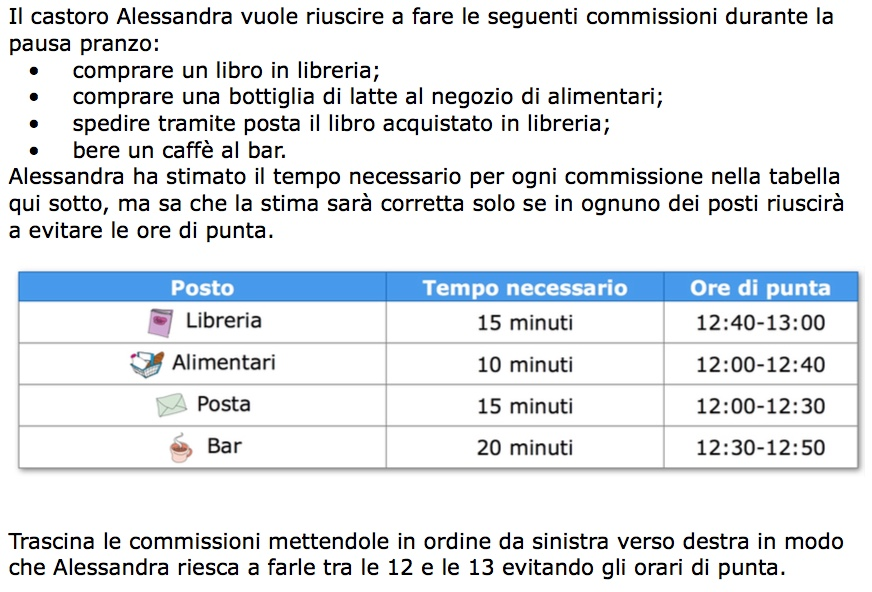
\includegraphics[height=10.0cm]{corrispondenze1.jpeg}}
	\caption{Commissioni (2016-LT-03)}\label{fig:4}
\end{figure}

Questo quesito può essere utilizzato ad esempio in relazione al seguente traguardo riportato tra le indicazioni della scuola primaria nell'area disciplinare di matematica:
“Ricerca dati per ricavare informazioni e costruisce rappresentazioni (tabelle e grafici). Ricava informazioni anche da dati rappresentati in tabelle e grafici.”
Lo studente per poter trovare l'ordine corretto delle commissioni, deve ricavare le informazioni dalla tabella data riguardanti il tempo necessario e le ore di punta da evitare. Una possibile strategia risolutiva è quella di creare a sua volta una tabella in cui indicare sulle righe le attività e la loro relativa durata e sulle colonne le possibili fasce orarie.

\begin{figure}[H]
	\centering
	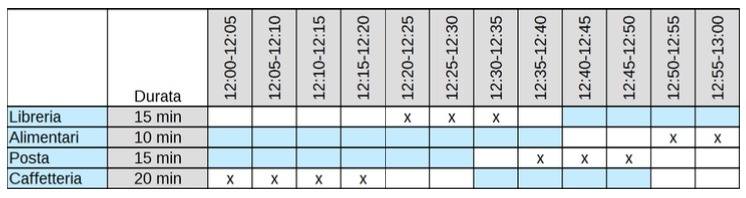
\includegraphics[height=4.0cm]{corrispondenze2.jpeg}
	\caption{Soluzione commissioni (2016-LT-03)}\label{fig:5}
\end{figure}

Anche nelle indicazioni della scuola secondaria di primo grado, area didattica di matematica, si possono trovare i seguenti traguardi:
"Analizza e interpreta rappresentazioni di dati per ricavarne misure di variabilità e prendere decisioni."
"Riconosce e risolve problemi in contesti diversi valutando le informazioni e la loro coerenza."
Lo studente deve interpretare la tabella proposta nel testo e dedurne le informazioni necessarie alla richiesta, inoltre deve valutare la compatibilità tra i vari eventi indicati per poterne decidere l'ordine.
"Spiega il procedimento seguito, anche in forma scritta, mantenendo il controllo sia sul processo risolutivo, sia sui risultati."
"Sostiene le proprie convinzioni, portando esempi e controesempi adeguati e utilizzando concatenazioni di affermazioni; accetta di cambiare opinione riconoscendo le conseguenze logiche di una argomentazione corretta."
Un possibile approfondimento didattico, successivo allo svolgimento del quesito alla classe, è quello di spiegare la costruzione della tabella da cui ricavare la soluzione e confrontare la strategia risolutiva proposta con quelle scelte dalle varie squadre partecipanti, incentivando in questo modo il confronto tra procedure e approcci diversi.

Tra gli obiettivi di apprendimento al termine della scuola secondaria di primo grado all'interno del nucleo tematico "Dati e previsioni", si possono individuare i punti che seguono.

"Rappresentare insiemi di dati, anche facendo uso di un foglio elettronico. In situazioni significative, confrontare dati al fine di prendere decisioni, utilizzando le distribuzioni delle frequenze e delle frequenze relative. Scegliere ed utilizzare valori medi (moda, mediana, media aritmetica) adeguati alla tipologia ed alle caratteristiche dei dati a disposizione. Saper valutare la variabilità di un insieme di dati determinandone, ad esempio, il campo di variazione."

\noindent Il docente può proporre come attività didattica di approfondimento, l'utilizzo di un foglio elettronico per rappresentare la tabella risolutiva introdotta precedentemente, e quindi avere un riscontro con la prima parte dell'obiettivo riportato sopra.

"Riconoscere coppie di eventi complementari, incompatibili, indipendenti."

\noindent Quest'ultimo punto è strettamente riconducibile allo scopo del quesito, infatti allo studente è richiesto di ordinare gli eventi e quindi riconoscere che tipo di relazione intercorre tra di essi.

Anche nell'area disciplinare di scienze è possibile rintracciare dei riferimenti utili:
"Individua nei fenomeni somiglianze e differenze, fa misurazioni, registra dati significativi, identifica relazioni spazio/temporali."

\noindent Il processo risolutivo del quesito chiede allo studente di riconoscere le relazioni temporali tra gli eventi proposti.

Questo lavoro di ricerca di corrispondenze tra i quesiti Bebras e le indicazioni, è stato svolto in maniera sistematica per ogni punto dei traguardi e degli obiettivi affini all'Informatica, riportati nella sezione \ref{indicazioni}, con lo scopo di mostrare come i quesiti Bebras possono essere una risorsa didattica all'interno di percorsi curricolari.

%%%%%%%%%%%



%%%%%%%%%%%%
%			CAPITOLO 3: CT e Bebras
\chapter{CT e Bebras}
\label{cap3}
%%%%%%%%%
\section{Cos'è il Computational Thinking}
% spiegazione del CT e riportare le operazioni del volantino del ciste

\section{Il Bebras e le abilità del pensiero computazionale}

%vedi articolo prof
%intervista docenti

%%%%%%%%%%%%
%			CAPITOLO 4: APPLICAZIONE WEB
\chapter{Applicazione web per il supporto didattico attraverso i quesiti Bebras}
\section{Tecnologie utilizzate}
\section{Applicazione web}


%%%%%%%%%%
%			BIBLIOGRAFIA
%
\begin{thebibliography}{00}
%
\bibitem{BellettiniITICSE2015}
C. Bellettini, V. Lonati, D. Malchiodi, M. Monga, A. Morpurgo, M. Torelli, 
"How challenging are Bebras tasks? An IRT analysis based on the performance of Italian students", 
Proceedings of the 2015 ACM Conference on Innovation and Technology in Computer Science Education (ITiCSE 2015), 
pp. 27-32, 
Lithuania, 
July, 6-8, 
2015.
%
\bibitem{DagieneIFIP2010}
V. Dagiene, G. Futschek, 
"Introducing Informatics Concepts through a Contest", 
IFIP working conference: New developments in ICT and education, 
Amiens: Universite de Picardie Jules Verne, 
2010.
%
\bibitem{LonatiITICSE2017}
V. Lonati, D. Malchiodi, M. Monga, A. Morpurgo, 
"Bebras as a teaching resource: classifying the tasks corpus using computational thinking skills", 
Proceedings of the 22nd annual conference on innovation and technology in computer science education (ITiCSE 2017) 
Bologna, Italy, 
2017.
%
\bibitem{DagieneISEEP2008}
V. Dagiene, G. Futschek, 
"Bebras international contest on informatics and computer literacy: Criteria for good tasks", 
ISSEP 2008, 
LNCS, vol. 5090, 
pp. 19–30, 
2008.
%
\bibitem{DagieneINFORMATICA2017}
V. Dagiene, S. Sentence, G. Stupuriene, 
"Developing a Two-Dimensional Categorization System for Educational Tasks in Informatics", 
Informatica, vol. 28, no.1, 
pp.23-44, 
2017.
%
\bibitem{flayerCT}
International Society for Technology in Education \& Computer Science Teachers Association, 
"Operational definition of computational thinking for K-12 education."
\url{https://csta.acm.org/Curriculum/sub/ CurrFiles/CompThinkingFlyer.pdf}, 
2011.
%
\bibitem{DagieneISSEP2016}
V. Dagiene, S. Sentance, 
"It’s computational thinking! bebras tasks in the curriculum", 
ISSEP 2016, 
LNCS, vol. 9973, 
pp. 28–39, 
2016.
%
\bibitem{indicazioniNazionali}
Indicazioni nazionali riguardanti gli obiettivi specifici di apprendimento concernenti le attività e gli insegnamenti compresi nei piani degli studi previsti per i percorsi liceali di cui all'art. 10, comma 3, del DPR 15/3/2010, n. 89, in relazione all'art. 2, commi 1 e 3, del medesimo regolamento, 2010.
%
\bibitem{DagieneKEYCIT2015}
V. Dagiene, G. Stupuriene, 
"Informatics education based on solving attractive tasks through a contest", 
KEYCIT 2014 - Key Competencies in Informatics and ICT, 
pp. 97 – 115, 
2015.
%
\bibitem{HabermanACM2011}
B. Haberman, A. Cohen, V. Dagiene, 
"The beaver contest: attracting youngsters to study computing", 
Proceedings of the 16th annual joint conference on Innovation and technology in computer science education, ACM, 
p. 378, 
2011.
%
\bibitem{LonatiISSEP2017}
V. Lonati, M. Monga, A. Morpurgo, D. Malchiodi, A. Calcagni, 
"Promoting computational thinking skills: would you use this Bebras task?", 
Proceedings of the international conference on informatics in schools: situation, evolution and perspectives (ISSEP2017) (in stampa) 
Helsinki, Finland, 
2017.
%
\bibitem{KalasIFIP2009}
I. Kalaš, M. Tomcsányiová, 
"Students’ Attitude to Programming in Modern Informatics", 
IFIP World Conference on Computers in Education, 
Bento Goncalves, Brazil, 
2009.
%
\bibitem{PohlLNCS2015}
W. Pohl, J. Westmeyer, 
"Content categories for informatics tasks", 
LNCS, vol.9378, 
pp. 61-62,
2015. 
%
\bibitem{SchwillEATCS1994}
A. Schwill, 
"Fundamental ideas of computer science", 
EATCS-Bulletin, vol. 53, 
pp. 274– 295, 
1994.
%
\bibitem{LonatiKoli2017}
V. Lonati, D. Malchiodi, M. Monga, A. Morpurgo, 
"How presentation affects the difficulty of computational thinking tasks: an IRT analysis", 
Proceedings of the 17th koli calling international conference on computing education research (in stampa),
Koli, Finland, 
2017.
%
\bibitem{BellettiniISSEP2014}
C. Bellettini, V. Lonati, D. Malchiodi, M. Monga, A. Morpurgo, M. Torelli, L. Zecca,
"Extracurricular activities for improving the perception of Informatics in Secondary schools",
Proceedings of ISSEP 2014 - 7th International conference on informatics in Schools: Situation, Evolution, and Perspective, 
Lecture Notes in Computer Science, 
vol. 8730, pp. 161-172,
Istanbul,
22-25 September 
2014.
%
\bibitem{BellettiniTOCE2014}
C. Bellettini, V. Lonati, D. Malchiodi, M. Monga, A. Morpurgo, M. Torelli, L. Zecca,
"Informatics Education in Italian Secondary Schools",
ACM Transactions on Computing Education (TOCE), 
vol. 14, issue 2,
June 
2014.
%
\bibitem{Mirolo2003}
Claudio Mirolo, "Quale informatica nella scuola?", \url{http://nid.dimi.uniud.it/pages/materials/discussion/ educazione.pdf} ,2003.
%
\bibitem{RoyalSociety2012}
The Royal Society, "Shut down or restart? The way forward for computing in UK schools", \url{http: //royalsociety.org/education/policy/computing-in-schools/report/}, 2012.
%
\bibitem{InformaticaScuola}
Programma il futuro, "Perché l'informatica nelle scuole",
\url{https://www.programmailfuturo.it/progetto/perche-partecipare/informatica-e-scuola}
%
\bibitem{IndicazioniLicei}
Indicazioni nazionali riguardanti gli obiettivi specifici di apprendimento concernenti le attività e gli insegnamenti compresi nei piani degli studi previsti per i percorsi liceali di cui all'art. 10, comma 3, del DPR 15/3/2010, n. 89, in relazione all'art. 2, commi 1 e 3, del medesimo regolamento, \url{http://nuovilicei.indire.it/content/index.php?action=lettura_paginata&id_m=7782&id_cnt=10497}, 2010.
%
\bibitem{IndicazioniIstituti}
Istituti professionali, linee guida per il passaggio al nuovo ordinamento, \url{http://www.indire.it/lucabas/lkmw_file/nuovi_tecnici///INDIC/_LINEE_ GUIDA_TECNICI_.pdf}, \url{http://www.indire.it/lucabas/lkmw_file/nuovi_professionali///linee_guid a/_LINEE GUIDA ISTITUTI PROFESSIONALI_.pdf}, 2010.
%
\bibitem{BellettiniTFA2015}
C. Bellettini, V. Lonati, D. Malchiodi, M. Monga, A. Morpurgo, F. Pedersini, "La formazione degli insegnanti della classe 42/A --- Informatica: l'esperienza dell'Università degli Studi di Milano", 
E questo tutti chiamano informatica, L'esperienza dei TFA nelle discipline informatiche, 
Collana Manuali 14 Sapienza Università Editrice Roma, Italia,
2015.
\end{thebibliography}
% 
%			RINGRAZIAMENTI
%
\prefacesection{Ringraziamenti}
asdjhgftry.
\end{document}


 
